% Presentación TP final — Pronóstico de viento en Potrerillos
% Compilar: tectonic presentacion.tex
\documentclass[12pt,aspectratio=169,t]{beamer}

\usetheme{Madrid}
\usecolortheme{seahorse}
\setbeamertemplate{navigation symbols}{}
\setbeamertemplate{footline}[frame number]

\usepackage{graphicx}
\usepackage{booktabs}

\graphicspath{{figs/}}

\title{Pronóstico de viento en Potrerillos}
\subtitle{Análisis de Series de Tiempo y Pronósticos}
\institute{UNSaM}
\date{12 de junio de 2026}
\author{Marcos Achaval \and Lucas Achaval}

\begin{document}

% ---------- Portada (no cuenta) ----------
\begin{frame}
  \titlepage
\end{frame}

% ---------- Slide 1: datos del grupo ----------
\begin{frame}{Datos del grupo}
  \begin{itemize}
    \item \textbf{Grupo:} 9
    \item Marcos Achaval --- \texttt{machavalrodriguez@unsam-bue.edu.ar}
    \item Lucas Achaval --- \texttt{lachavalrodriguez@estudiantes.unsam.edu.ar}
    \vspace{0.8em}
    \item \textbf{Título:} Pronóstico de viento en Potrerillos
    \item \textbf{Dataset:} \url{https://www.windguru.cz/station/15338}
  \end{itemize}
\end{frame}

% ---------- Slide 2: problema ----------
\begin{frame}{Problema y objetivo}
  \begin{itemize}
    \item Potrerillos, Mendoza --- \textbf{viento térmico}
    \item Estación Ecowitt WS90 (club náutico)
    \item Endógena: viento promedio (nudos)
    \item Exógenas: viento máximo, temperatura, humedad, presión, dirección
    \vspace{0.5em}
    \item Objetivo: pronóstico a \textbf{12 horas} (1 predicción por hora)
  \end{itemize}
\end{frame}

% ---------- Slide 3: datos ----------
\begin{frame}{Datos}
  \begin{itemize}\itemsep0pt
    \item \textbf{Ago 2025 $\to$ abr 2026} ($\sim$8.5 meses) · 1 dato/min $\to$ \textbf{resampleo 1\,h} (6145 obs)
    \item Mediana (lineales) · \textbf{media circular} (dirección)
    \item Faltantes: 4.5\,\%, 12 gaps de estación $\to$ \textbf{sin imputar}
  \end{itemize}
  \vspace{0.6em}
  \centering
  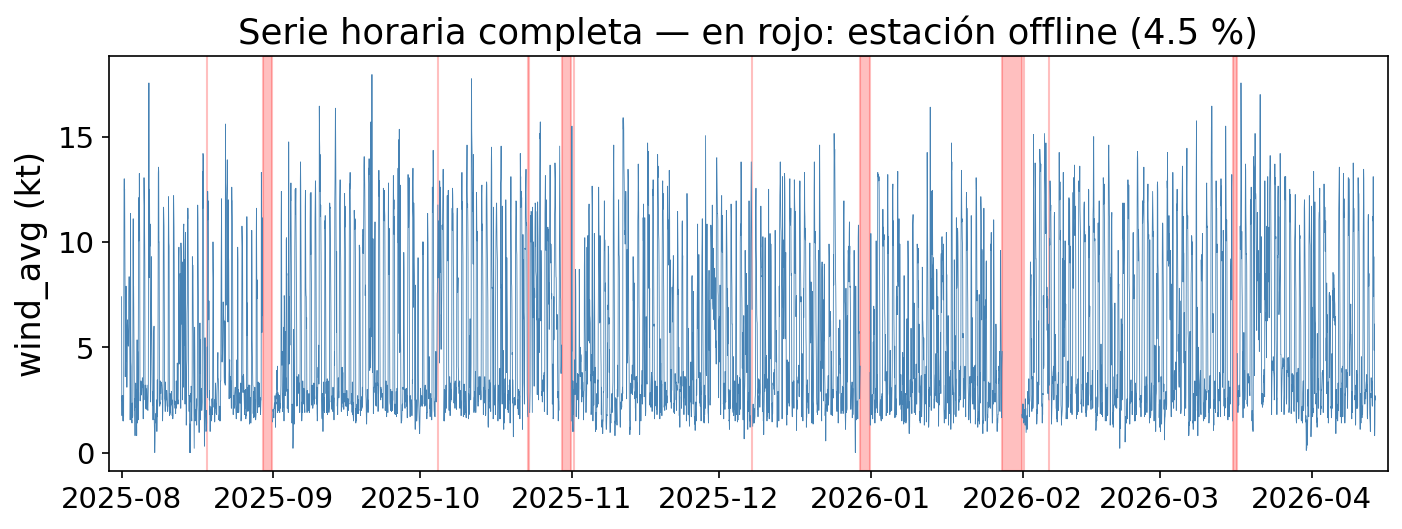
\includegraphics[width=\textwidth,height=0.54\textheight,keepaspectratio]{serie_completa.png}
\end{frame}

% ---------- Slide 4: EDA ciclo diurno ----------
\begin{frame}{EDA: ciclo diurno}
  \begin{itemize}\itemsep0pt
    \item Ciclo térmico diario: calma nocturna $\sim$1--2 kt · pico 11--16\,h
    \item Sin tendencia de largo plazo
  \end{itemize}
  \vspace{0.6em}
  \begin{columns}
    \column{0.4\textwidth}
      \centering
      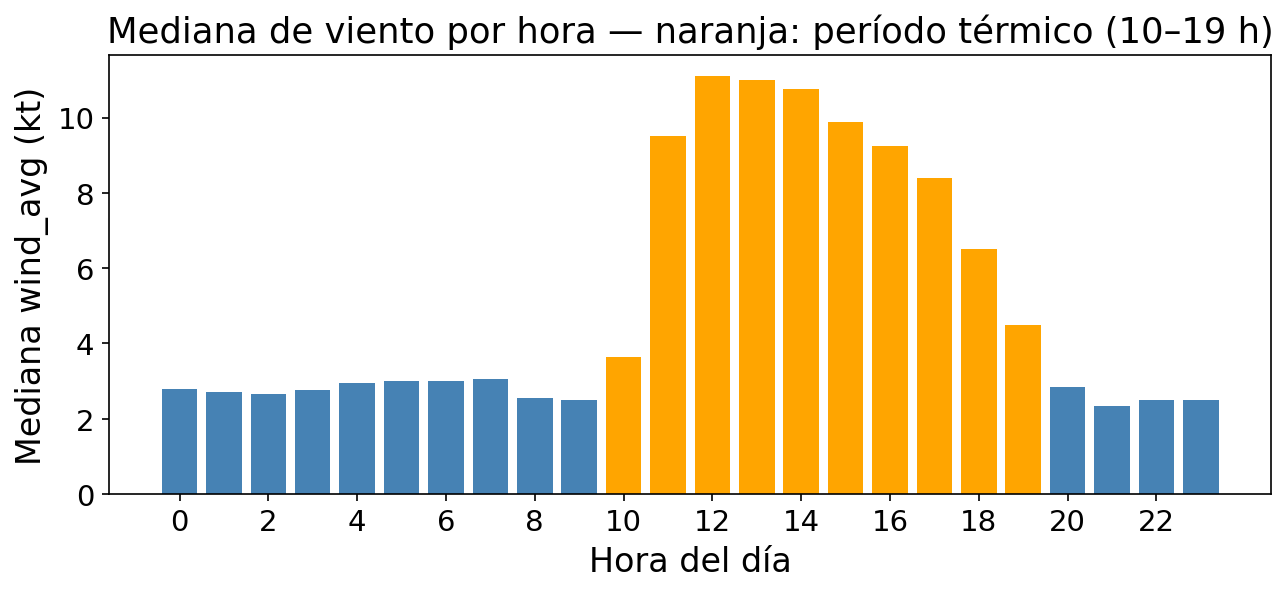
\includegraphics[width=\textwidth,height=0.66\textheight,keepaspectratio]{mediana_hora.png}
    \column{0.6\textwidth}
      \centering
      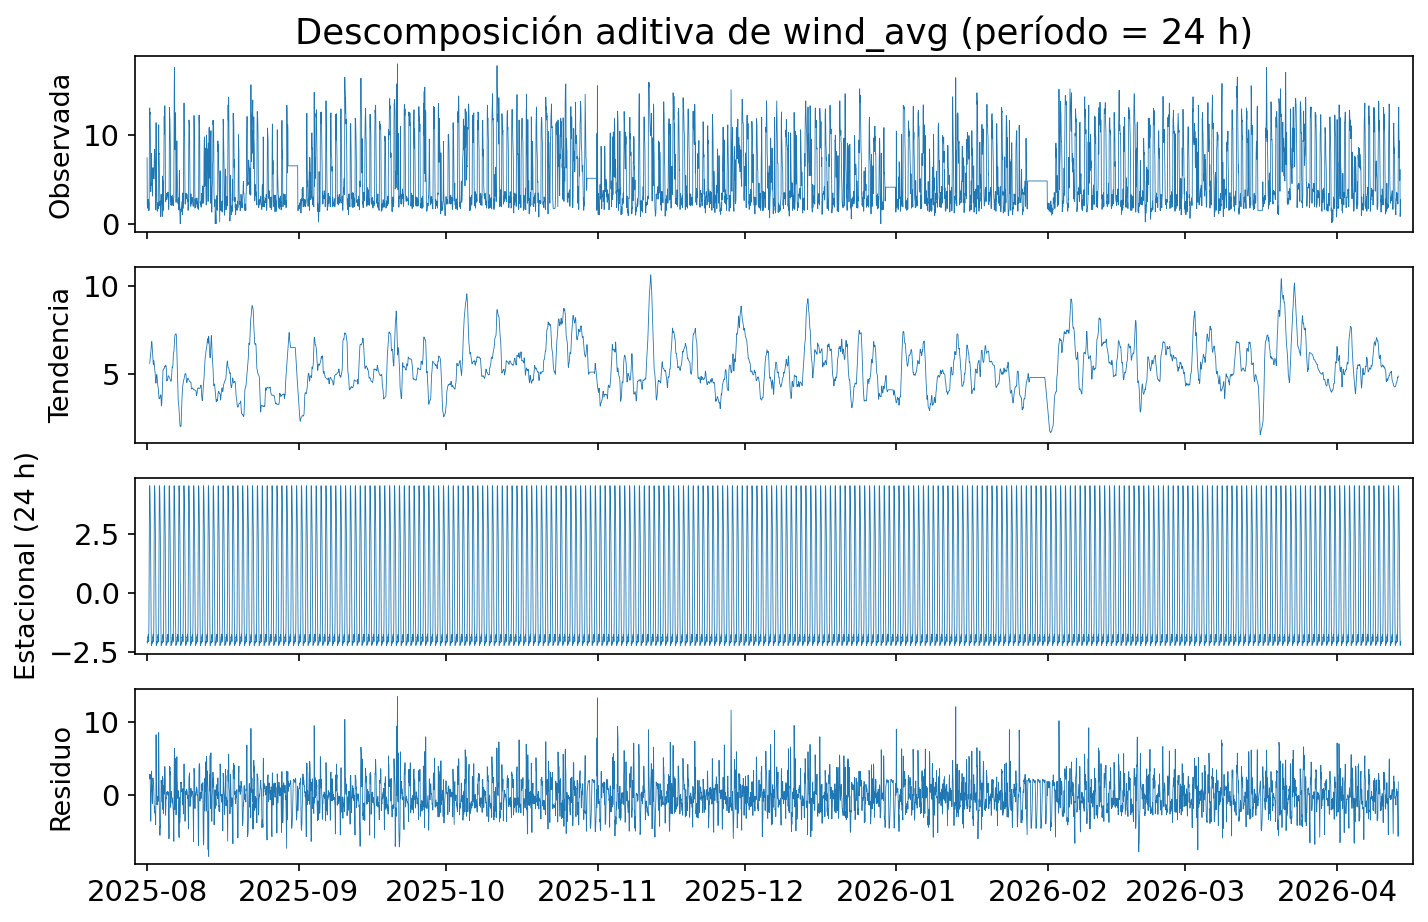
\includegraphics[width=\textwidth,height=0.66\textheight,keepaspectratio]{descomposicion.png}
  \end{columns}
\end{frame}

% ---------- Slide 5: ACF/PACF ----------
\begin{frame}{ACF/PACF y estacionariedad}
  \begin{itemize}\itemsep0pt
    \item ACF lag 24: $+0.5$ · lag 12: negativo (espejo día/noche)
    \item PACF: solo lags \textbf{1--2 y 20--24}
    \item ADF: $p \approx 7.58\times10^{-21}$ $\to$ \textbf{estacionaria} (sin diferenciar)
  \end{itemize}
  \vspace{0.6em}
  \centering
  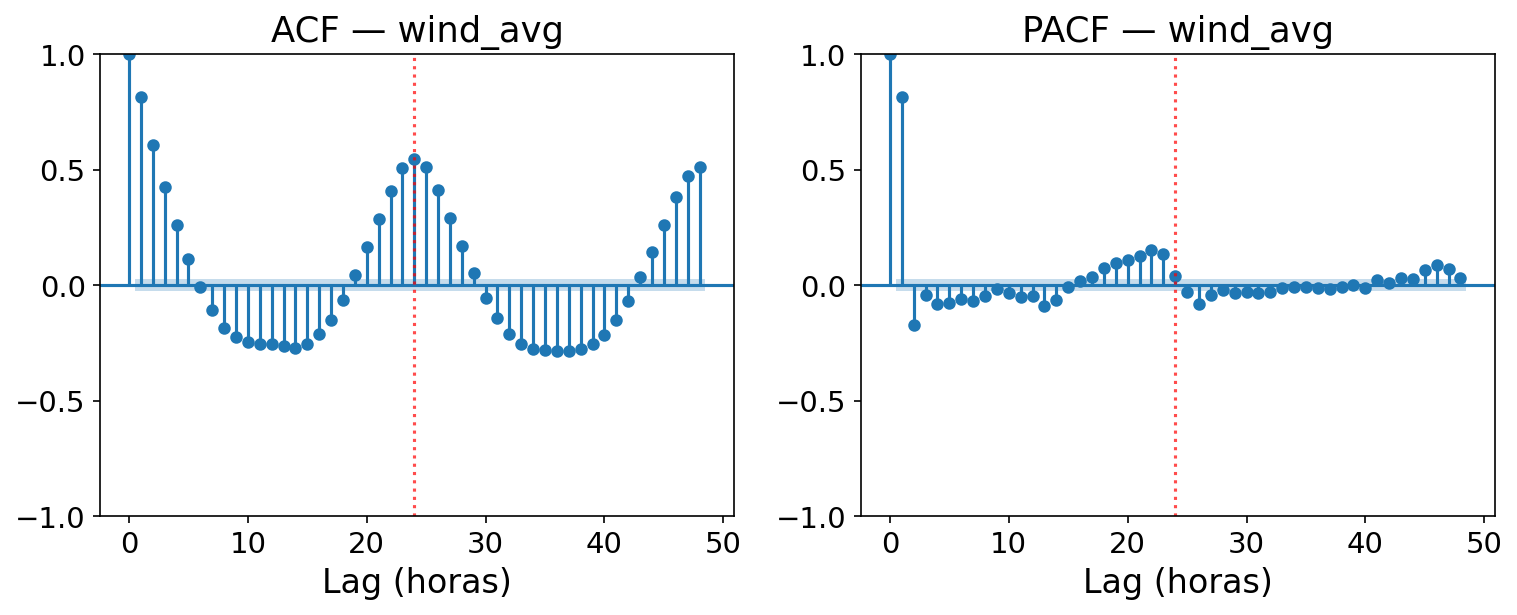
\includegraphics[width=\textwidth,height=0.62\textheight,keepaspectratio]{acf_pacf.png}
\end{frame}

% ---------- Slide 6: frecuencia ----------
\begin{frame}{Dominio de la frecuencia}
  \begin{itemize}\itemsep0pt
    \item Pico dominante: \textbf{1 ciclo/día} · secundario débil: 2 ciclos/día
    \item Sin periodicidades multi-día $\to$ forzante térmico puro, $S=24$
  \end{itemize}
  \vspace{0.6em}
  \centering
  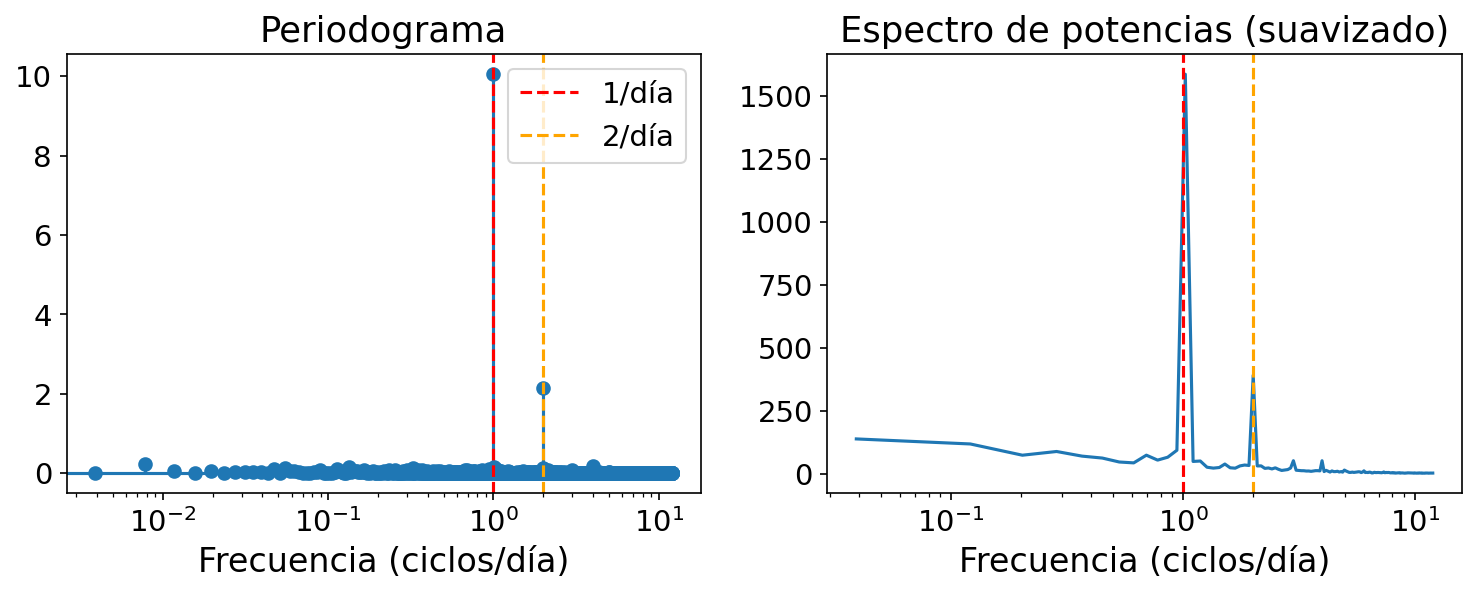
\includegraphics[width=\textwidth,height=0.6\textheight,keepaspectratio]{periodograma.png}
\end{frame}

% ---------- Slide 7: metodologia + benchmark ----------
\begin{frame}{Metodología y benchmark}
  \begin{itemize}\itemsep0pt
    \item Walk-forward · $h = 1\ldots12$ · MAE / RMSE / $R^2$ por horizonte · split 80/20
    \item Benchmark: \textbf{persistencia estacional} $\;\hat{y}_{t+h} = y_{t+h-24}$
    \item RMSE \textbf{3.6 kt} · MAE 2.6 kt · $R^2$ 0.17
  \end{itemize}
  \vspace{0.6em}
  \centering
  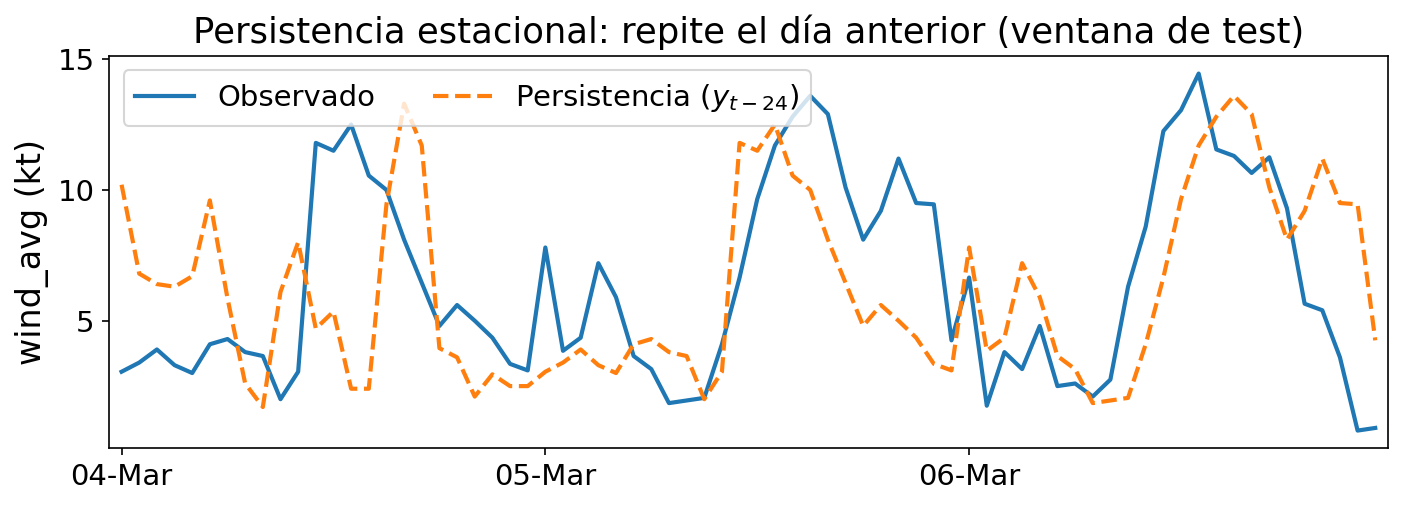
\includegraphics[width=0.85\textwidth,height=0.54\textheight,keepaspectratio]{obs_vs_persistencia.png}
\end{frame}

% ---------- Slide 8: LassoCV ----------
\begin{frame}{Modelo de ML: LassoCV}
  \begin{itemize}\itemsep0pt
    \item 31 features: \textbf{24 lags} + 5 exógenas + \textbf{sin/cos hora}
    \item L1 $\to$ selección automática · RMSE \textbf{2.8 kt} ($-24\,\%$) · $R^2$ 0.52
  \end{itemize}
  \vspace{0.6em}
  \begin{center}
    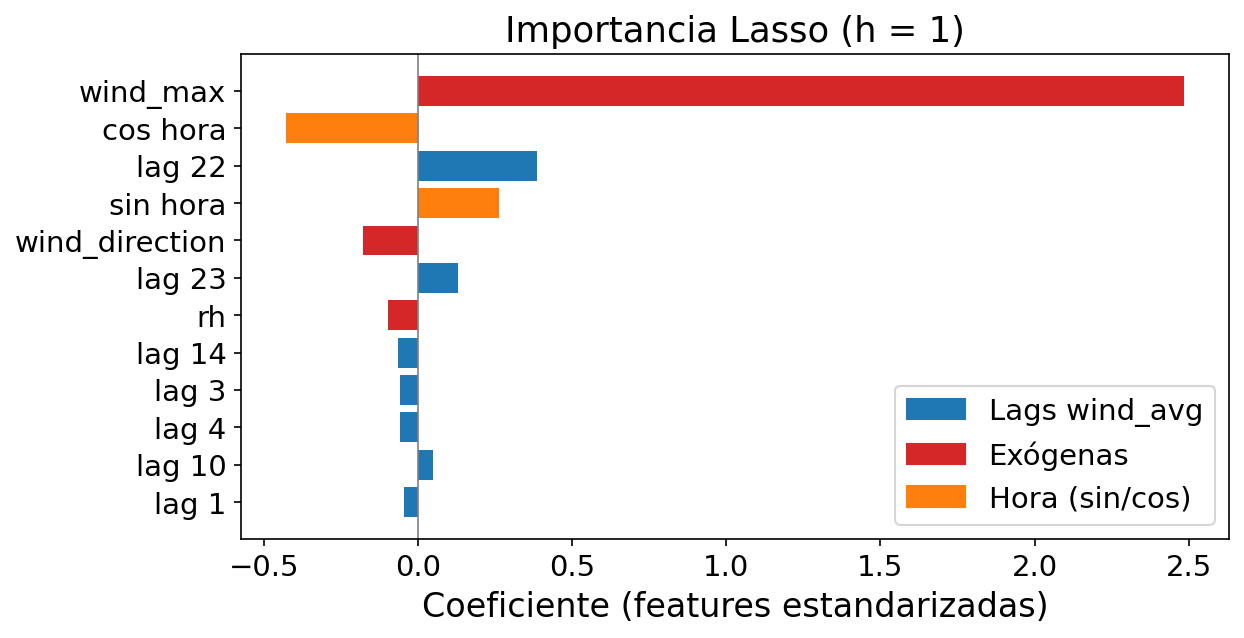
\includegraphics[height=0.46\textheight]{lasso_importancia.png}\hspace{0.6em}%
    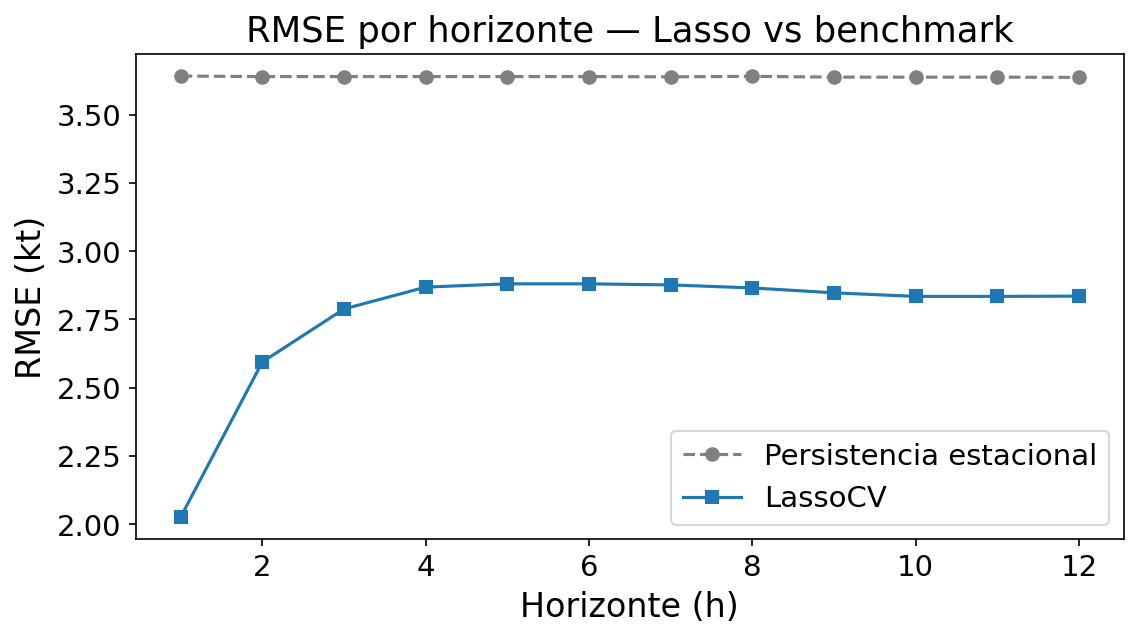
\includegraphics[height=0.46\textheight]{lasso_vs_bench.png}
  \end{center}
\end{frame}

% ---------- Slide 9: SARIMA seleccion ----------
\begin{frame}{Modelo superador: SARIMA --- selección}
  \begin{itemize}\itemsep4pt
    \item ACF/PACF $\to$ AR corto + estacional $S=24$, $d=D=0$
    \item Grid search por \textbf{AIC}: $p \in \{0,1,2\}$ · $q \in \{0,1\}$ · $P,Q \in \{0,1\}$
    \item Elegido: \textbf{SARIMA$(2,0,1)(1,0,1)_{24}$}
  \end{itemize}
  \vspace{2em}
  \centering
  \small
  \setlength{\tabcolsep}{14pt}
  \begin{tabular}{ccccr}
    \toprule
    $p$ & $q$ & $P$ & $Q$ & AIC \\
    \midrule
    \textbf{2} & \textbf{1} & \textbf{1} & \textbf{1} & \textbf{20496} \\
    1 & 1 & 1 & 1 & 20501 \\
    2 & 0 & 1 & 1 & 20504 \\
    1 & 0 & 1 & 1 & 20515 \\
    2 & 1 & 1 & 0 & 21167 \\
    \bottomrule
  \end{tabular}
\end{frame}

% ---------- Slide 10: SARIMA diagnostico ----------
\begin{frame}{SARIMA: diagnóstico y resultados}
  \begin{itemize}\itemsep0pt
    \item Ljung-Box \checkmark{} · Q--Q: \textbf{colas pesadas}
    \item RMSE \textbf{2.6 kt} ($\mathbf{-28\,\%}$) · $R^2$ 0.57 · $h{=}1$: $R^2$ 0.78
  \end{itemize}
  \vspace{0.6em}
  \centering
  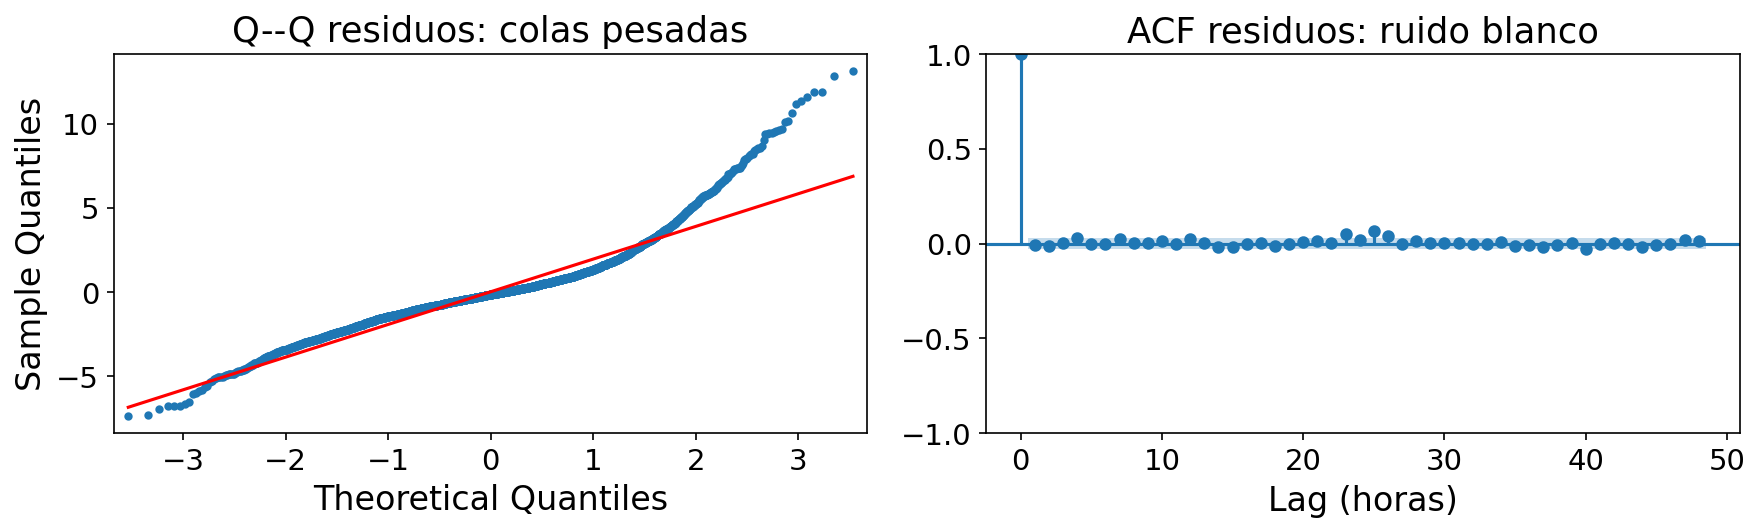
\includegraphics[width=\textwidth,height=0.66\textheight,keepaspectratio]{sarima_diag2.png}
\end{frame}

% ---------- Slide 11: redes ----------
\begin{frame}{Alternativas: redes neuronales --- RMSE por horizonte}
  \begin{itemize}\itemsep0pt
    \item Dense / LSTM · ventana $W{=}48$ · salida directa $H{=}12$
    \item LSTM: RMSE \textbf{2.8 kt} --- no supera a SARIMA
  \end{itemize}
  \vspace{0.6em}
  \centering
  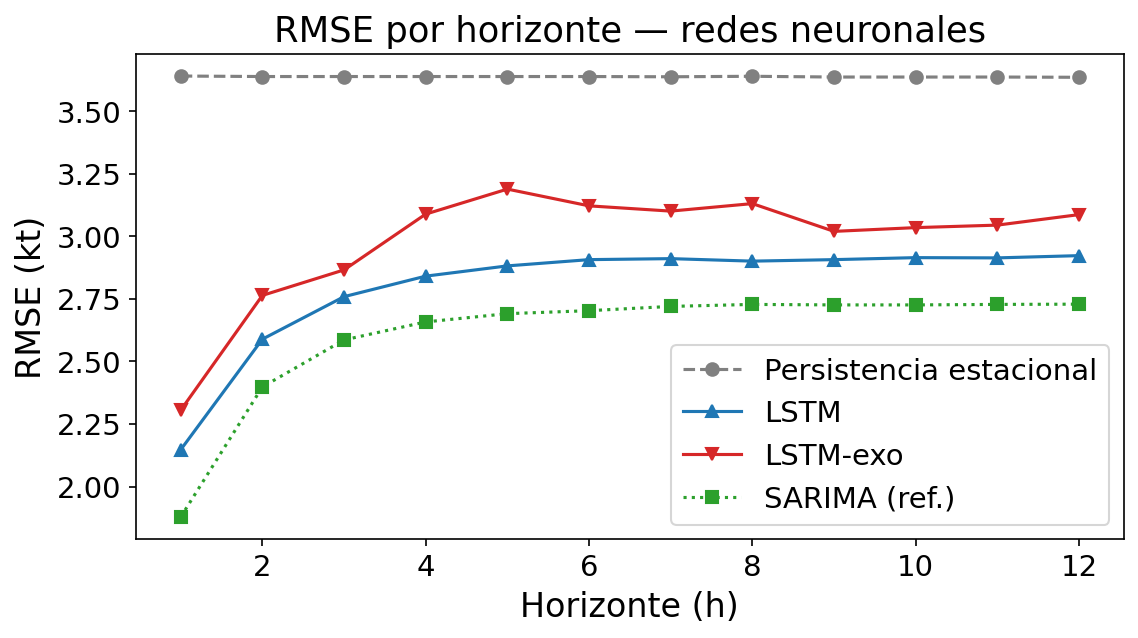
\includegraphics[width=\textwidth,height=0.66\textheight,keepaspectratio]{nn_vs_bench.png}
\end{frame}

% ---------- Slide 11b: redes (val vs test) ----------
\begin{frame}{Alternativas: redes neuronales --- validación vs test}
  \begin{itemize}\itemsep0pt
    \item Exógenas pasadas \textbf{no aportan} a resolución horaria
  \end{itemize}
  \vspace{0.6em}
  \centering
  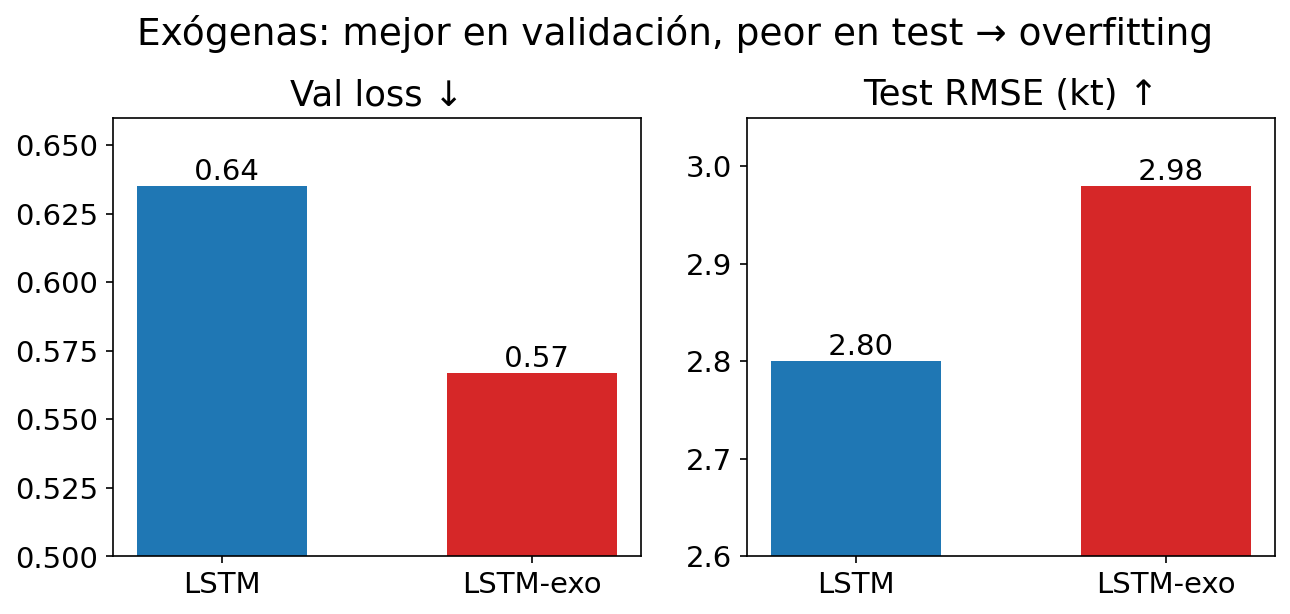
\includegraphics[width=\textwidth,height=0.68\textheight,keepaspectratio]{nn_overfit.png}
\end{frame}

% ---------- Slide 12: comparacion final ----------
\begin{frame}{Comparación final}
  \centering
  \footnotesize
  \begin{tabular}{lcccc}
    \toprule
    Modelo & MAE (kt) & RMSE (kt) & $R^2$ & $\Delta$ RMSE \\
    \midrule
    \textbf{SARIMA$(2,0,1)(1,0,1)_{24}$} & \textbf{1.9} & \textbf{2.6} & \textbf{0.57} & $\mathbf{-28\,\%}$ \\
    Lasso & 2.1 & 2.8 & 0.52 & $-24\,\%$ \\
    LSTM & 2.1 & 2.8 & 0.51 & $-23\,\%$ \\
    LSTM-exo & 2.3 & 3.0 & 0.44 & $-18\,\%$ \\
    Persistencia estacional & 2.6 & 3.6 & 0.17 & --- \\
    \bottomrule
  \end{tabular}
  \vspace{0.6em}

  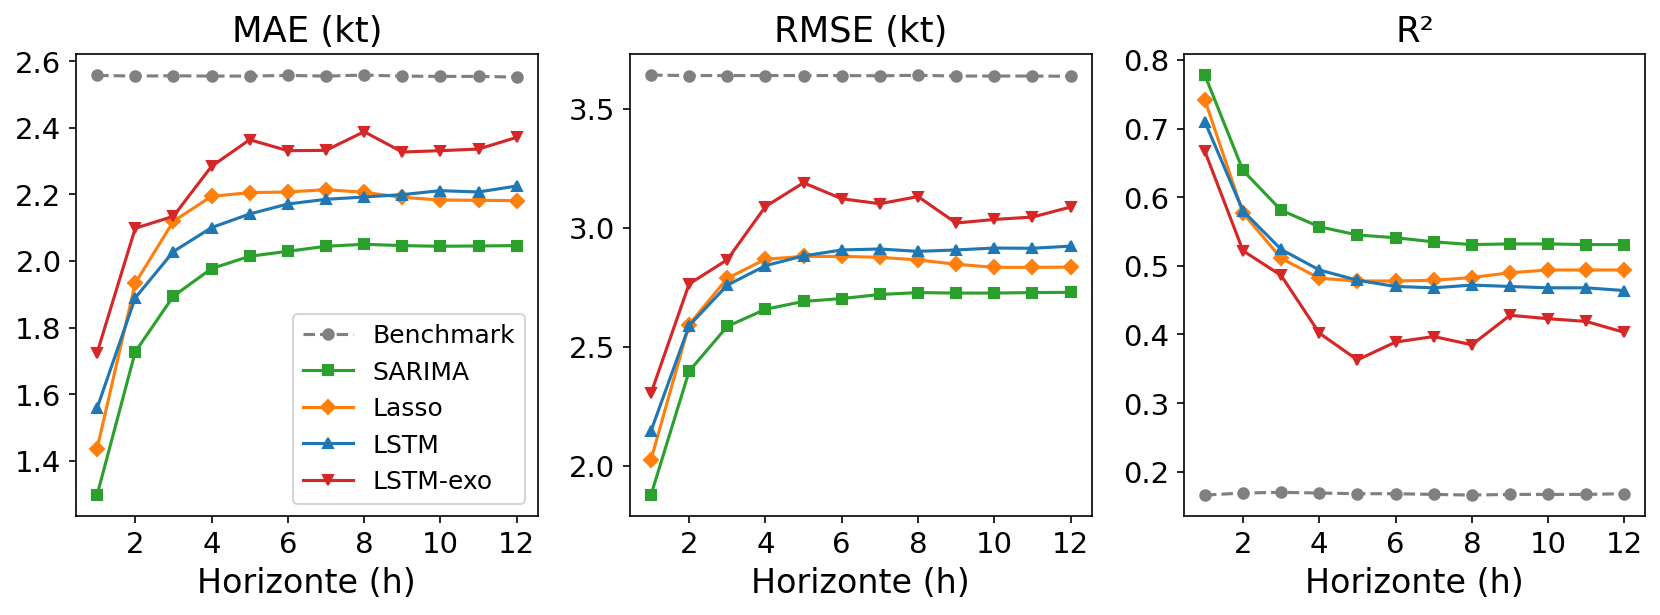
\includegraphics[width=\textwidth,height=0.46\textheight,keepaspectratio]{comparacion_final.png}
\end{frame}

% ---------- Slide 13: conclusiones ----------
\begin{frame}{Conclusiones y trabajo futuro}
  \textbf{Conclusiones}
  \begin{itemize}\itemsep2pt
    \item Viento térmico $\approx$ reloj: \textbf{ciclo 24\,h domina}
    \item \textbf{SARIMA}: $-28\,\%$ RMSE, simple y suficiente
    \item Exógenas pasadas: no mejoran
  \end{itemize}
  \vspace{0.6em}
  \textbf{Trabajo futuro}
  \begin{itemize}\itemsep2pt
    \item \textbf{SARIMAX}
    \item \textbf{GARCH} $\to$ intervalos honestos
    \item Encoding circular de dirección
    \item Exógenas \textbf{pronosticadas} (NWP)
  \end{itemize}
\end{frame}

% ---------- Slide final: agradecimiento ----------
\begin{frame}[plain,c]
  \centering
  {\Huge \textbf{¡Gracias!}}\\[1em]
  {\Large ¿Preguntas?}
\end{frame}

\end{document}
